\chapter{Kapcsolódó tanulmányok}
Ennek a fejezetnek célja, hogy összefoglaljam a diplomamunkámhoz előzetesen elvégzett kutatómunka során megismert tanulmányok eredményeit, problémáit, valamint a lehetséges alkalmazásukat.

A kutatómunkámat három témában végeztem, az első a fenyegetésmodellezés (threat modeling) területe volt. Ezen kutatásokon keresztül ismertem meg a fenyegetések felmérése során felmerülő problémákat, megoldásuknak módjait, azok lehetséges megjelenítését és modellezését.

A második téma az autóipari biztonsági elemzések területén készült munkák kutatása volt, hogy meg tudjam ismerni milyen komponenseket és azoknak mely attribútumai lesznek használhatóak egy elemzés során. Szintén tartalmaztak a kutatások olyan metodológiákat és best practice-eket amelyeket a saját analízis metodológiám során is fel tudtam használni.

A harmadik, utolsó és egyben a legspecifikusabb téma, a már meglévő kutatások amelyek támadási fák (attack trees), illetve támadási gráfok (attack graphs) generálásáról szóltak, ezek az üzembiztonság területén elterjedt hibafa (fault tree) analízis eszközének adaptációi a kiberbiztonsági terület támogatására.

\section{Fenyegetésmodellezés}

Az első témába illő kutatás a Karahasanovic et al.\cite{Karahasanovic} kutatása volt "Adapting Threat Modelling Methods for the Automotive Industry" címmel. Ez két fenyegetésmodellezési keretrendszert mutat be, egyik az Intel-hez köthető TARA (Threat Agent Risk Assessment), ami nem összekeverendő az azonos rövidítéssel fémjelzett Threat Analysis and Risk Assessment metodológiával amit az ISO 21434 definiál, a másik pedig, a sokkal ismertebb Microsoft által fejlesztett STRIDE. 

Az előbbi a grafikus modellezési technikák helyett egy könyvtárakon alapuló fenyegetés elemzést mutat be, ahol három könyvtárat használnak, egyik a lehetséges támadó ágenseket, másik az általuk véghezvihető támadásokat a harmadik pedig, a jellemző támadási felületeket gyűjti. 

A kutatás ezen könyvtárakból határoz meg egy részhalmazt ami az autóipari rendszerek ellen alkalmazható. A második technika már a támadó-centrikusság helyett inkább szoftver-centrikus irányt követi, ami egy fehér doboz vizsgálatot tesz lehetővé a rendszeren. Ez, a későbbiekben még előforduló Data Flow Diagramok használatára mutat be egy példát amelyben a szoftver komponensek közti kommunikációt modellezi és tud egy támadási útvonalat végigkövetni. 

Az előbbi technika gyengesége az, hogy csak magas szinten definiálja a fenyegetéseket ami nem elégséges a védelmi mechanizmusok meghatározására. Utóbbi ezzel szemben alkalmas arra, viszont nem lehet vele rendszer szintű védelmet modellezni, valamint tervezési fázisban is nehezen alkalmazható.\\

Ma et al.\cite{Ma} kutatása "Threat Modeling for Automotive Security Analysis" címmel, a fenyegetésmodellezést egy sokkal gyakorlatibb módon közelíti meg, nem feltétlenül a technikai részekre koncentrál, hanem a termékfejlesztési életciklust és a már meglévő üzembiztonsági analíziseket is figyelembe veszi. 

Helyesen jelzi a szükségét az analízis szintekre bontásának, hasonlóan az üzembiztonsághoz, azonosítja az igényét egy funkcionális kiberbiztonsági tervnek valamint egy technikai kiberbiztonsági tervnek, kiegészítve egy termékspecifikációval. Ezeknek a jelenlétét pedig lebontja az elsőt a tervezési fázisban, magas szintű követelmények azonosításához, a másodikat termékfejlesztési szakaszhoz, bemenetként a rendszermodellt használva, a specifikációt pedig gyártási fázisban való használattal. 

A kutatás tartalmaz még egy esettanulmányt amely, egy jármű utasterének a biztonsági analízisén vezet végig, a Microsoft Threat Modelling Tool használatával, ami a STRIDE keretrendszerre épít, data flow diagramokat használ és modell alapon generál lehetséges fenyegetéseket. 

Konklúzióként emeli ki az igényt, hogy a biztonsági analízis modellezési paradigmáit, valahogyan integrálni szeretnék a rendszermodellezés paradigmáival, ezzel biztosítva, hogy az analízis a változások során napra kész maradjon. A termékfejlesztési fázisok és kiberbiztonsági elemzéseket a \ref{fig:MA} ábrán részletezik.\\

\begin{figure}[!ht]
\centering
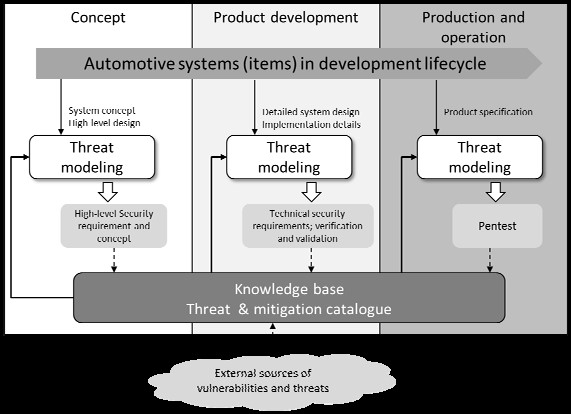
\includegraphics[width=125mm, keepaspectratio]{figures/03_MA.png}
\caption{Fenyegetésmodellezés a termékfejlesztési életciklusokban\cite{Ma}}
\label{fig:MA}
\end{figure}

Ehhez a területhez tartozik még Vivek et al.\cite{Vivek} kutatása ami egy esettanulmány volt, egy tetszőleges autóipari komponensre, kiértékeléshez egy módosított STRIDE modellt használt, valamint az ISO 21434-ben definiált kockázatelemzés kezdeti lépéseit amelyek a lehetséges fenyegetések feltárására vannak alkalmazva.

\section{Kiberbiztonság és üzembiztonság kapcsolata}

Ezzel a témával kapcsolatban Dantas et al. \cite{Dantas} kutatása mutatja be, hogy a szabványosított kockázatelemzésre, hogyan lehet már meglévő technikákat alkalmazni valamint, hogy a kockázatelemzés, hogyan illeszkedik be már létező folyamatokba. 

A dokumentum részletesen elemzi a kiberbiztonság fontosságát az autóiparban, valamint a szoftverfrissítés jelenlétét mint fontos eszközt esetleges sérülékenységek javításában. Szintén elemezve van a rendszeres és folyamatos auditálása és kiértékelése ezeknek a folyamatoknak. Ezekhez jelzi a lehetőséget különböző domén-specifikus nyelvek használatának lehetőségét és automatizálás integrálását, illetve modellellenőrző rendszerek bevezetését. 

Van még szó az üzembiztonság területén alkalmazott FTA (Fault Tree Analysis) és FMEA (Failure Modes and Effects Analysis) technikájának felhasználásáról a támadási útvonalak elemzésében, illetve idéz több más tanulmányt és keretrendszert amelyek szintén ezen alkalmazásokat ösztönzik.\\

Bohner et al.\cite{Bohner} kutatása az üzembiztonsági architektúrát terjesztené ki a kiberbiztonsági kockázatok kezelésére. Helyesen hívja fel a figyelmet arra, hogy a kiberbiztonsági elemzések alapjául használt CIA triádból kettő, az integritás (integrity) valamint a rendelkezésre állás (availability) az üzembiztonság területén már véletlenszerű hibák esetére alkalmazva vannak. 

Említésre kerülnek itt a memória particionálás mint ami a két területen csökkentik a kockázatot, az üzenetek védelmét módosítás ellen, valamint összességében a kiberbiztonság mint részhalmaza az üzembiztonságnak ahol a véletlenszerűen előforduló hibák helyett a szándékosan okozott hibákat kell figyelembe vennünk. A kockázat csökkentő intézkedések alkalmazása pedig szignifikánsan tudja mind a két fajta biztonság hatékony szolgáltatását.\\

Chulp et al.\cite{Chulp} kutatása egy ThreatGet nevezetű kiberbiztonsági kockázatelemző eszköz működési elvét mutatja be amely a bécsi egyetemen készült. Ez az eszköz gyakorlatiasan írja le a tervezési fázisban elvégzendő kockázatelemzés menetét, ebben már az ASPICE-szal ellentétben láthatunk feedback alkalmazását a folyamat lépései közt és egy külön modellt is használ kockázatelemzésre amelyet össze hasonlítana a meglévő rendszermodellel, ahogy az a \ref{fig:CHULP} ábrán látható.

Chulp et al.\cite{Chulp} kutatásában továbbá hasonlóan az én munkámhoz a STRIDE fenyegetésmodellezési keretrendszert valamint a CIA triád közös használatát végzik el. Szintén érdemes kiemelni a fenyegetésmodellezésre jellemzően használt Data Flow diagram kiegészített formáját amelyet Extended Data Flow diagramnak neveznek, ebben egy részről kompozíciók modellezését teszik lehetővé, másrészről pedig értékek (asset) megjelenítéséről is gondoskodtak. Ez a modell már sokkal alkalmasabb komplex kiber-fizikai rendszerek elemzésére az általános Data Flow diagrammokkal szemben. Ez a diagram a \ref{fig:CHULP_EDD} ábrán látható.

\begin{figure}[!ht]
	\centering
	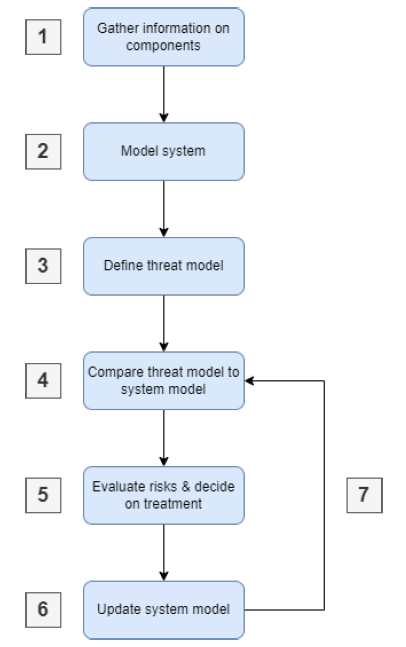
\includegraphics[width=75mm, keepaspectratio]{figures/03_CHULP.png}
	\caption{Fenyegetésmodellezés folyamata a tervezési fázisban\cite{Chulp}}
	\label{fig:CHULP}
\end{figure}

\begin{figure}[!ht]
	\centering
	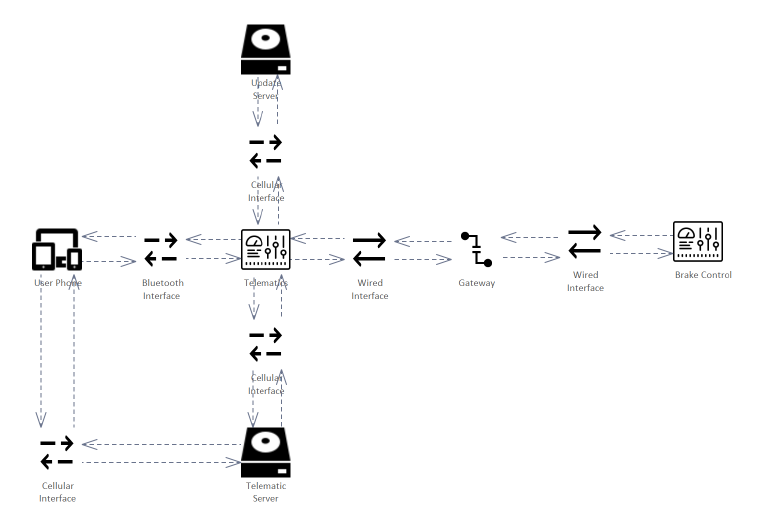
\includegraphics[width=125mm, keepaspectratio]{figures/03_CHULP_EDD.png}
	\caption{Extended Data Flow diagram grafikus megjelenítése\cite{Chulp}}
	\label{fig:CHULP_EDD}
\end{figure}

Ebben a kutatásban hangzik el először az automatizált támadási fa generálásának fogalma, valamint a tanulmány támadási gráfokat is definiál. A kutatás jól használja fel az Extended Data Flow Diagram rendszermodelljét támadási fák és gráfok generálására amelyekből támadási utakat vezet le amelyek alkalmasak lesznek valódi kockázatok meghatározására.

Magukról a támadási fákról alkotott modell pedig a \ref{fig:CHULP_AT} ábra mutatja be. Ezen nehezen látható, hogy az Extended Data Flow diagramból (ami a \ref{fig:CHULP_EDD} ábrán látható) lenne származtatva a modell, valamint a végeredmény egy absztrakt megfogalmazású és nem kifejezetten az egyes komponensekre irányuló támadásokat jelenít meg a támadás lépéseiként. Szintén a dependenciák is kevésbé használják ki a logikai kapuk nyújtotta felépítés lehetőségeit.

\begin{figure}[!ht]
	\centering
	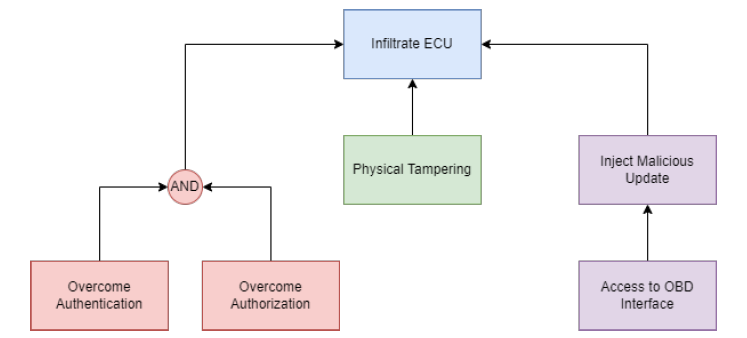
\includegraphics[width=125mm, keepaspectratio]{figures/03_CHULP_AT.png}
	\caption{Támadási fák grafikus megjelenítése\cite{Chulp}}
	\label{fig:CHULP_AT}
\end{figure}

\section{Támadási fa generálás}

Sowka et al.\cite{Sowka} publikációja különböző alkalmazásait értékelte az automatikus támadási fáknak az autóipari kiberbiztonság doménjében. Az írás ad egy általános áttekintést a terület fontosságáról, a szabályozási környezet aktuális helyzetéről majd összehasonlította a különböző elérhető megoldásokat az adott problémára.

A Salfer et al.\cite{Salfer} kutatása által bemutatott módszer egy magas fokú modellezett megoldás alapján való támadási utak előállítását határozza meg. Kifejezetten érdekes, ahogy felépíti a metamodelljét amiben definiál egy rendszer és egy támadó modellt is. A rendszermodell meghatározza az elektronikus vezérlő egységeket, szoftvereket, kommunikációs hálózatokat és értékeket (\textit{asset}), a támadó modell pedig tartalmazza a tudást, motivációt, amelyek aztán a támadások megvalósíthatóságának értékelésében játszanak szerepet. Szintén elemzi ezeknek a támadási utaknak az alkalmazását a rendszer kiberbiztonsági (penetrációs) tesztelésénél és jól ismeri fel, hogy ez egy magasszintű white-box tesztelésben lehetne felhasználható. 

Karray et al.\cite{Karray} kutatása sokban épít az előző bekezdésben említettre, azonban itt nem lehet egy explicit támadómodellről beszélni. A rendszermodell használ bizonyos tulajdonságokat amelyek jelzik a támadó szükséges tudását vagy belépési szükségét, viszont kevesebb feltevést használ a támadások meghatározásánál. A gráf trnaszformáció valamint a rendszermodell még alkalmas lehet a saját munkámhoz.

Végül pedig Bryans et al.\cite{Bryans} kutatását néztem meg amely kombinálja a modell alapú valamint a könyvtár alapú automatizált generálást, azaz a modell és template alapú támadási fa generálást. A Chulp et al.\cite{Chulp} kritikája alapján is ez volt kiemelve mint legérettebb megoldás, valamint ez is az egyik legfiatalabb. A támadó modell helyett előredefiniált támadási mintákat használ fel, amelyek segítségével rekurzívan tud a fa leveleiből kifejteni komplexebb támadásokat egyfajta bottom-up megközelítésben. A rendszermodell szemben a template-ekkel sokkal egyszerűbb, nem különít el ECU funkcionalitást vagy értékeket, emiatt ez a része nem lesz használható a munkám során, viszont ez teszi lehetővé teszteléskor a black-box megközelítést, valamint akár teszt kódok és eszközök integrációjával is lehetne használni deszkriptív template-ek esetén. Célom az, hogy ezt a fajta kombinált megközelítést alkalmazzam erősebben rendszermodellezett megközelítéssel és egyszerűsítettebb template-ekkel.
